


The first geometric model tested is the \emph{ratio model}. The main idea behind this model is to reproduce the observed polarization morphologies, ranging from purely aligned with the minor axis of the disk to purely azimuthal, along with intermediate cases. This was achieved by creating a grid of models weighted between these two extreme cases. 

The first extreme case is a 100\% uniform pattern, where every vector is aligned with the minor axis of the disk (90\degg from the disk position angle, Table \ref{tab: source_info}).  This is shown in the left panel of Figure \ref{fig: RatioExamples}. The second extreme case is a 100\% azimuthal pattern, where the polarization vectors follow a circular pattern around the centre of the disk. The centre point of the disk at each wavelength can be found in Table \ref{tab: source_info}. For each pixel $(x, y)$, the offset from the disk centre $(x_c, y_c)$ is calculated as:
\begin{equation}
\begin{aligned}
    \delta x &= x - x_c, \\
    \delta y &= y - y_c.
\end{aligned}
% \label{eq: vectors}
\end{equation}


\noindent These offsets are then used to calculate the azimuthal polarization angle using \texttt{numpy.arctan2}. This is shown in the right panel of Figure \ref{fig: RatioExamples}.



To create the intermediate cases, models were generated in steps of 10\% and are denoted as $N \uni + (100 - N) \azi$, where $N = 0, 10 \ldots, 100$. Here, Uni and Azi represent the pure uniform and pure azimuthal cases, respectively, and $N$ gives the percentage contribution of the uniform case. 

Since the polarization angles cannot be directly combined, the \SQ and \SU for the extreme cases ($100\uni+0\azi$ and $0\uni+100\azi$) were calculated from the polarization angle grids using:

\begin{equation}
\begin{aligned}
Q_{\text{Uni}} &= \rho I \cos(2\theta_{\text{Uni}}) \text{ and }
Q_\text{Azi} = \rho I \cos(2\theta_\text{Azi}),
     \\
U_{\text{Uni}} &=  \rho I \sin(2\theta_{\text{Uni}}) , \text{ and }
U_\text{Azi} =  \rho I \sin(2\theta_\text{Azi}) 
\end{aligned}
% \label{eq:50U50A}
\end{equation}
\noindent following \cite{Montier}, where $\rho$ is the average polarization fraction over the centre and edges, which fixed at 2\%. This value is expected to be reasonable for the uniform polarization morphology, but the polarization fraction may differ for the azimuthal morphology, potentially biasing the azimuthal case low.

%This is consistent with values of 0.02-0.03 from \cite{Kataoka_2017}, 



The intermediate \SQ and $U$ maps were then obtained by combining the two extreme models using:
\begin{equation}
\begin{aligned}
Q_{N}
    &= \frac{N}{100}\,Q_{\text{Uni}}
     + \frac{100 -N}{100}\,Q_{\text{Uni}}, \\
U_{N}
    &= \frac{N}{100}\,U_{\text{Uni}}
     + \frac{100 -N}{100}\,U_{\text{Azi}}.
\end{aligned}
% \label{eq:50U50A}
\end{equation}

\noindent The resulting $Q_N$ and $U_N$ model maps were used to calculate the model polarization angle at each pixel using Equation \ref{eq: PA}. The polarization vectors were generated using the methods in Chapter \ref{sec: chap4_polarization_vectors}. This process was repeated for each ratio combination. For example, $N=50$ corresponds to the $50\uni+50\azi$ model, shown in the middle panel of Figure \ref{fig: RatioExamples}.





\begin{figure}[htbp]
  \centering
  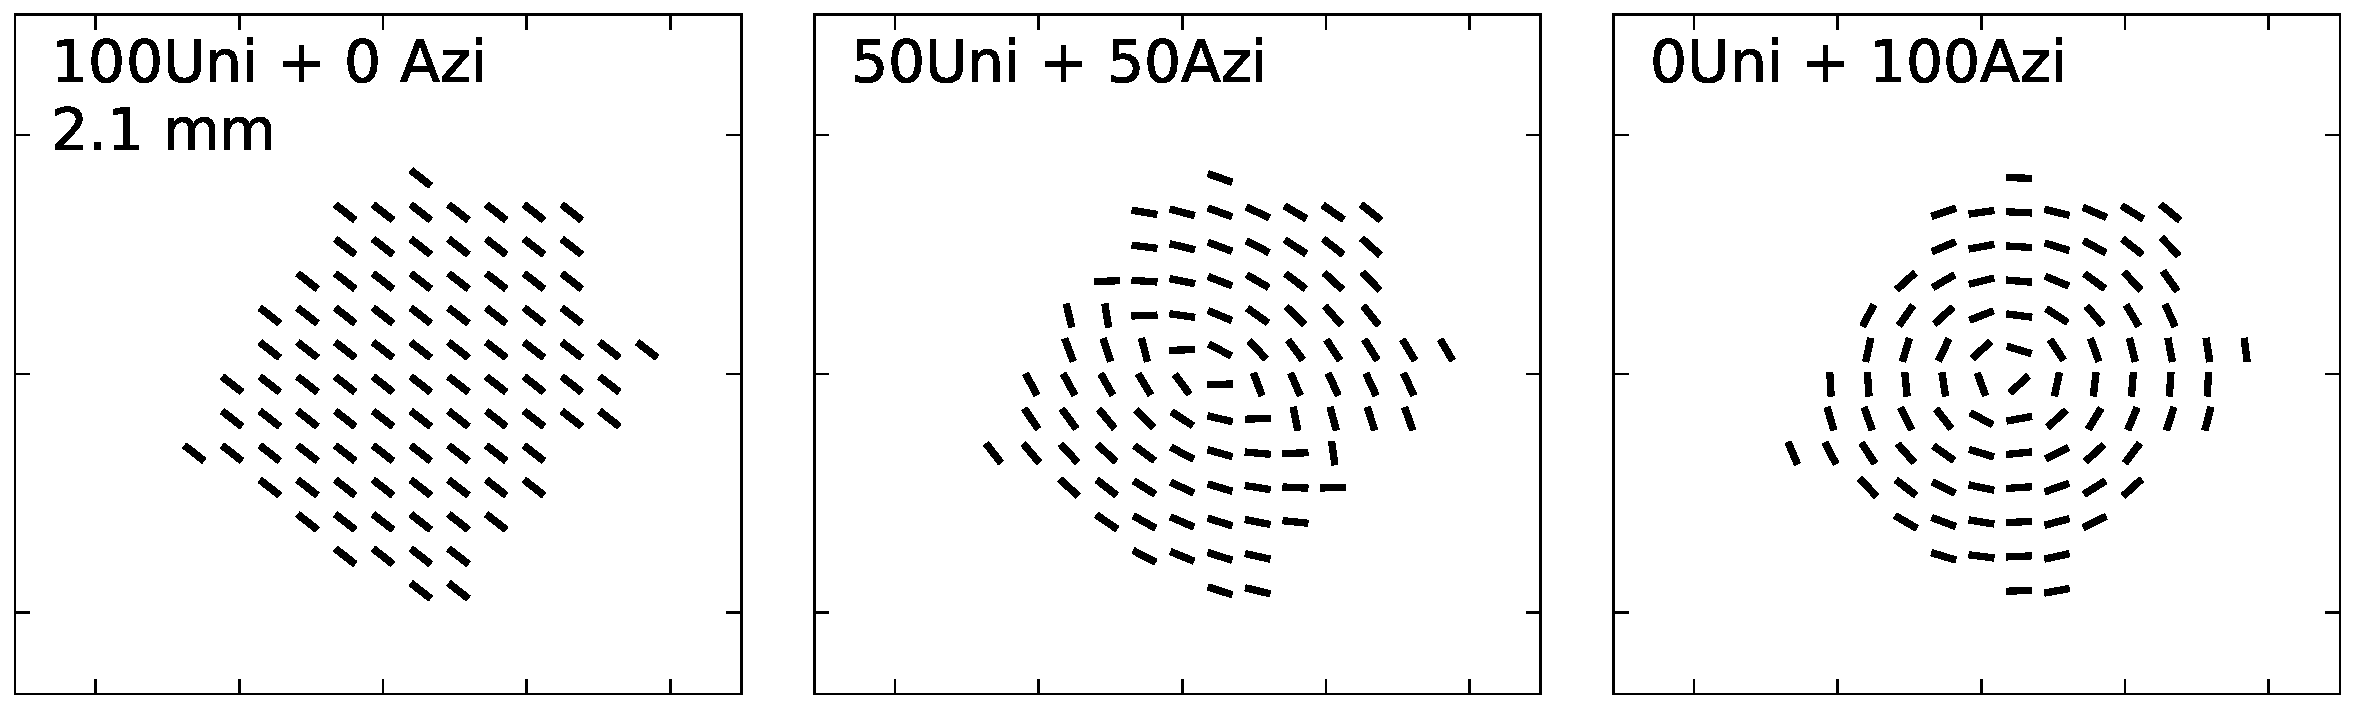
\includegraphics[width=0.99\textwidth]{WRITEUP_AND_IMAGES/IMAGES/WRITEUP/Ratio/RatioExamplesTest_Band4_NoAxes.pdf}
  \caption[Example of the $N = 100, N=50$ and $N = 0$ cases of the ratio model.]{Example of the $N = 100, N=50$ and $N = 0$ cases of the ratio model for \bfourNS.}
  \label{fig: RatioExamples}
\end{figure}





For the ratio models, Table \ref{tab:ratio_model_chi2} presents the \chired values calculated for each test with the best-fit value shown in bold.  Figure \ref{fig: RatioBestGrid} shows the best-fit model with the observed vectors in black and the model vectors in red.


Taking \bfive as an outlier (see Chapter \ref{sec: discussion_band5_data_issues}), the best-fit ratio models show that, as wavelength decreases, the observations are better matched with a higher uniform contribution. This result is consistent with the observations discussed in Chapter \ref{sec: c4_polarization_maps}, which show a greater uniform contribution with decreasing wavelength. 






% This was updated to Band 5 robust = -1 on July 18th
% These numbers might need to be changed if we change how we calculate chi^2
% This is Band 4 nterms2, Band 7 nterms 2.
\begin{table}[h!]
\centering
\caption[Ratio model fitting results.]{Ratio model fitting results for each wavelength, with goodness-of-fit quantified by $\chi^2_{reduced}$. Best fits are shown in bold. }
\begin{tabular}{lcccc}
\toprule
\textbf{Ratio Model} & \textbf{\bfour} & \textbf{\bfive} & \textbf{\bsix} & \textbf{\bseven} \\
\midrule
100Uni + 0Azi
& 181.67 % Band 4 
& \textbf{22.58} % Band 5 
& 37.39 % Band 6  
& \textbf{79.12} \\


90Uni + 10Azi
& 171.40 % Band 4
& 24.22 % Band 5  
& 33.93 % Band 6  
& 88.59 \\

80Uni + 20Azi
& 158.01 % Band 4 
& 27.77 % Band 5  
& \textbf{33.36} % Band 6  
& 108.65 \\

70Uni + 30Azi
& 140.74 % Band 4 
& 34.28 % Band 5  
& 37.99 % Band 6 
& 144.84 \\

60Uni + 40Azi
& 116.11 % Band 4 
& 45.10 % Band 5
& 51.96 % Band 6 
& 206.76 \\

50Uni + 50 Azi
& \textbf{88.21} % Band 4 
& 63.81 % Band 5  
& 84.48 % Band 6  
& 322.01 \\

40Uni + 60Azi
& 124.99 % Band 4 
& 91.17 % Band 5  
& 140.41 % Band 6  
& 498.43 \\

30Uni + 70 Azi
& 131.03 % Band 4 
& 116.35 % Band 5
& 191.20 
& 647.50 \\

20Uni + 80Azi
& 133.70 % Band 4 
& 138.36 % Band 5  
& 233.90 % Band 6  
& 776.00 \\

10Uni + 90Azi
& 136.42 % Band 4
& 157.27 % Band 5  
& 270.41 % Band 6 
& 886.40 \\

0Uni + 100Azi
& 139.41
& 173.26
& 302.34 
& 979.97 \\
\bottomrule
\end{tabular}
% \begin{tablenotes}
% \footnotesize
% \item \textbf{Note:} Values of . 
% \end{tablenotes}
\label{tab:ratio_model_chi2}
\end{table}





% PLOTS
% ----------------------------------------
% ----------------------------------------
% \begin{figure*}[h]
%   \centering

%   % Row 1
%   \begin{minipage}{0.48\textwidth}
%     \centering
%     
\includegraphics[width=\linewidth]{IMAGES/WRITEUP/Ratio/IRS63_best_ratio_BAND4.pdf}
%     \textbf{(a) Band 4}
%   \end{minipage}
%   \hfill
%   \begin{minipage}{0.48\textwidth}
%     \centering
%     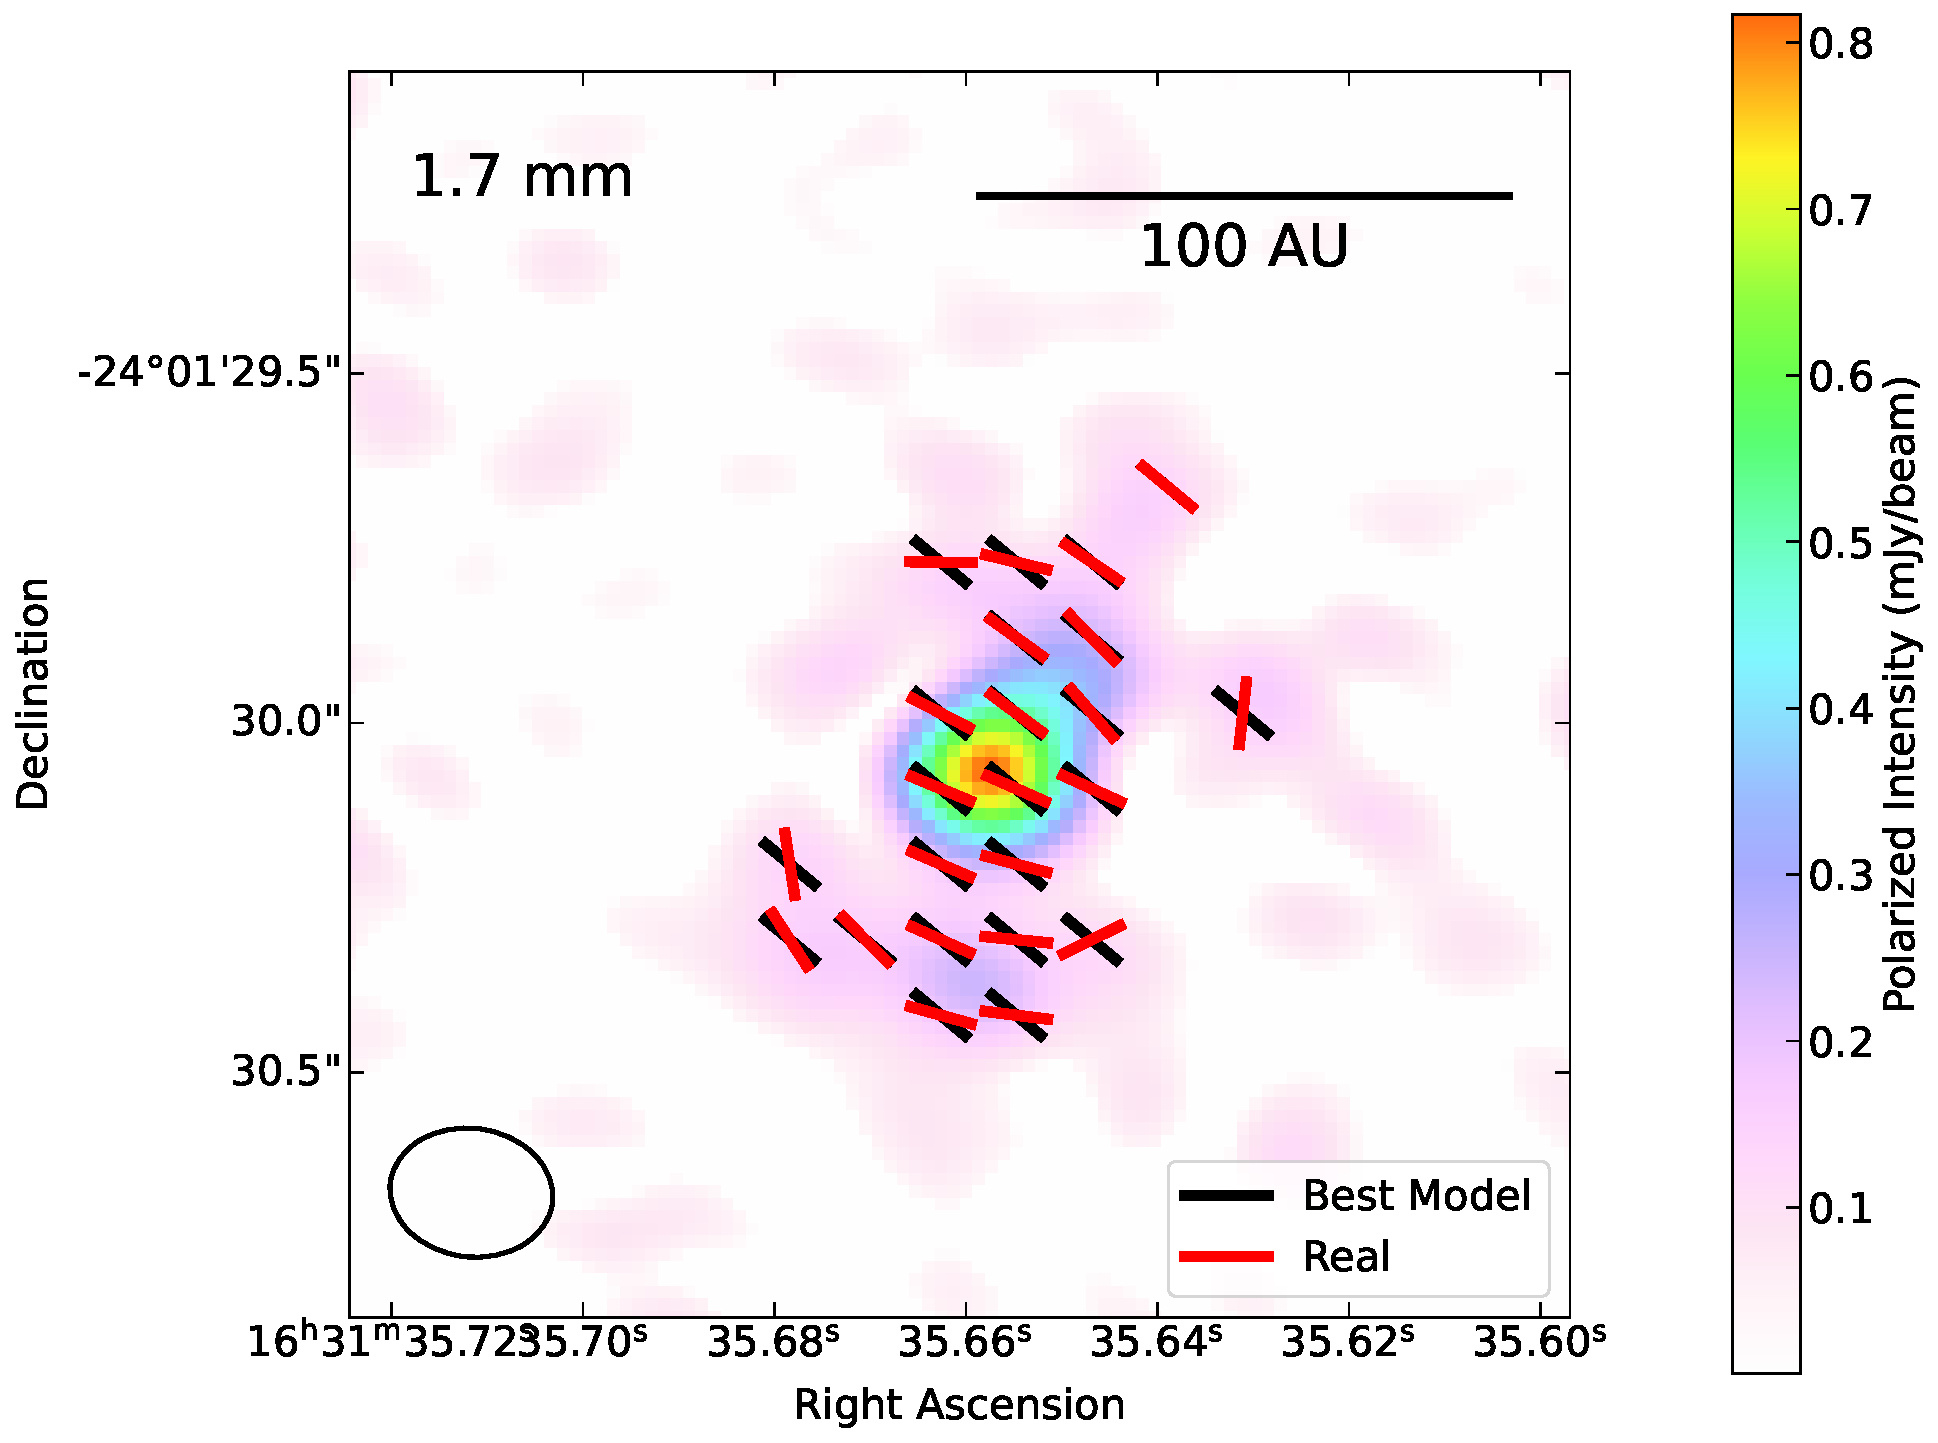
\includegraphics[width=\linewidth]{IMAGES/WRITEUP/Ratio/IRS63_best_ratio_BAND5_robust_minus1.pdf}
%     \textbf{(b) Band 5}
%   \end{minipage}

%   \vspace{0.5cm}

%   % Row 2
%   \begin{minipage}{0.48\textwidth}
%     \centering
%     \includegraphics[width=\linewidth]{WRITEUP_AND_IMAGES/
%   \end{minipage}
%   \hfill
%   \begin{minipage}{0.48\textwidth}
%     \centering
%     
\includegraphics[width=\linewidth]{IMAGES/WRITEUP/Ratio/IRS63_best_ratio_BAND7.pdf}
%     \textbf{(d) Band 7}
%   \end{minipage}

%   \caption{
%   \add{caption, make this a grid} \note{Change to $\Delta\alpha$ and $\Delta \delta$ if we chose to do that for other plots.} \note{Update to band 5 robust -1}
%   }

%   \label{fig:best-ratio-models}
% \end{figure*}
% ----------------------------------------
% ----------------------------------------





\begin{figure}[htbp]
  \centering
  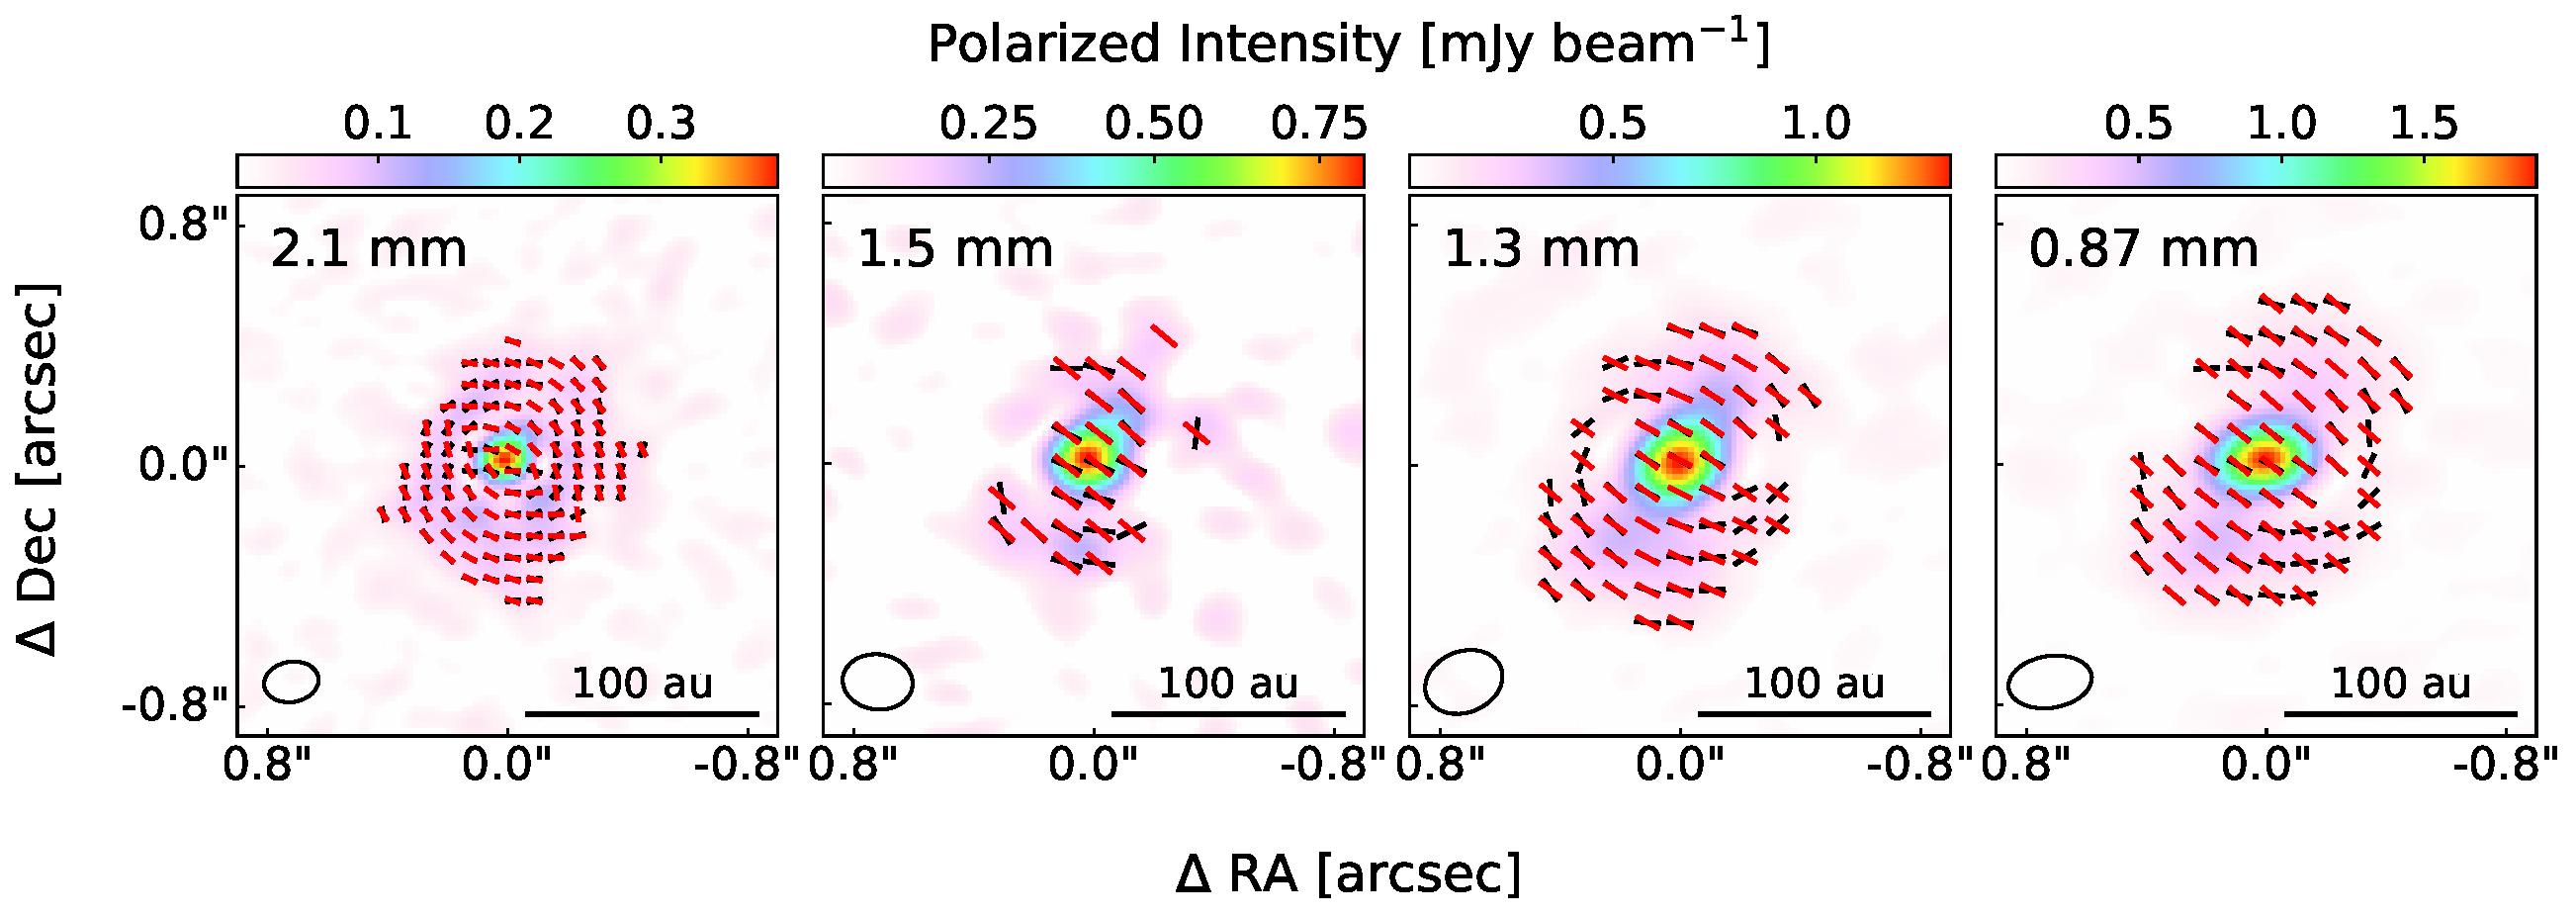
\includegraphics[width=0.99\textwidth]{WRITEUP_AND_IMAGES/IMAGES/WRITEUP/Ratio/Best_grid_Delta.pdf}
  \caption[Figure \ref{fig: StokesI_POLI_grid}, with the polarization vectors from the best-fit ratio model.]{Figure \ref{fig: StokesI_POLI_grid}, overplotted with the polarization vectors in red from the best-fit ratio model at each wavelength. The corresponding best-fit ratio models are listed in Table \ref{tab:ratio_model_chi2}.  }
  \label{fig: RatioBestGrid}
\end{figure}


